\documentclass{slides}
%
%babel
\usepackage[romanian]{babel}
%
\usepackage{graphicx}%dorim să importăm grafică
\usepackage{amsfonts}
\title{Legile lui Newton}
\author{Student\footnote{313AC}}
\date{}
\begin{document}
\maketitle
%\begin{abstract}
\textbf{Lucrarea prezintă ...}
%\end{abstract}
%
%\section{Introducere}\label{intro}
\begin{center}
\textbf{Introducere}
\end{center}
Lucrarea se bazează pe informația prezentată în \cite{wiki}....
%\section{Tratare}
\begin{center}
\textbf{Tratare}
\end{center}
Dintre principiile mentionate în secțiunea \ref{intro}, un loc remarcabil îl reprezintă legea a doua a dinamicii, descrisă de
\begin{equation}
\vec{F}=m\vec{a}
\end{equation}
Urmează tabelul de definire ....
%\begin{table}[htbp]
\centering
%\caption{Unități de măsura}\label{tab:unit}
\begin{tabular}{lll}
\hline
Nr.&Mărime&Unitate de măsură\\\hline
\end{tabular}
%\end{table}
Un grafic în figura \ref{fig:figura}...
%\begin{figure}[ht]
\centering
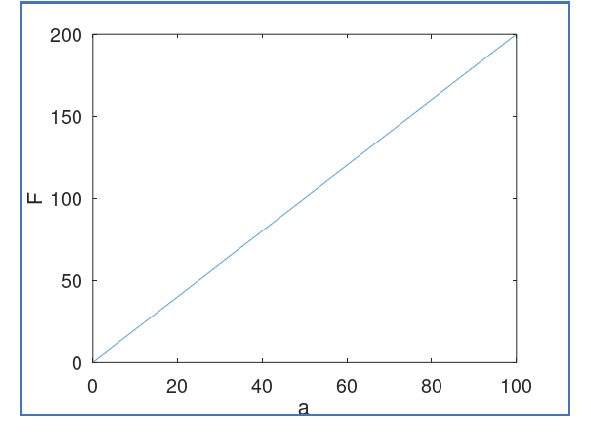
\includegraphics[scale=0.8]{figura.pdf}
\caption{Evoluția ...}\label{fig:figura}
%\end{figure}
\section{Concluzii}
\begin{thebibliography}{a}
\bibitem{wiki} Wikipedia-Legile lui Newton: \verb+https://ro.wikipedia.org/wiki/Legile_lui_Newton+
\end{thebibliography}
\end{document}